\raggedright

In order to further understand how a DDoS works and why it can be effectively unstoppable, we have to take a deeper look into the taxonomy of a DDoS attack.

\vspace{0.5cm}

Although there are a wide array of DDoS attacks, there are no specific methods a single attack would use - it all depends on the aim of the attack. Specht and Lee\textsuperscript{\cite{specht2003taxonomies}} proposed a taxonomy of the main DDoS attack vectors and describes that there are two primary classes of attacks: \textit{bandwidth depletion} and \textit{resource depletion}.

\vspace{0.5cm}

\begin{figure}[h]
\begin{center}
	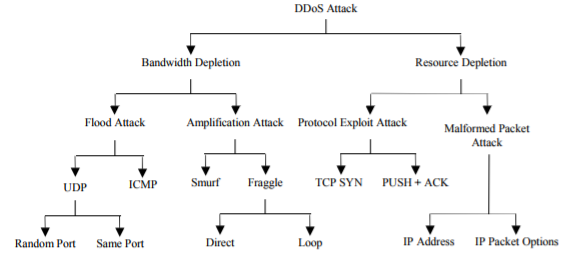
\includegraphics[width=0.75\textwidth]{img/ddos_attack_vectors.png}
	\caption{Taxonomy of a DDoS Attack}
\end{center}
\end{figure}

\vspace{0.5cm}

The most common types of attacks performed include:
\begin{itemize}
	\item{UDP, ICMP and SYN Floods}
	\item{TCP/SYN}
	\item{Zombie Attack}
\end{itemize}

\vspace{0.5cm}

Zombie attacks are not described in the taxonomy provided by Specht and Lee\textsuperscript{\cite{specht2003taxonomies}}, however they are an important mention. This type of attack occurs when non-spoofed connections overload services, causing network paralysis. These are extremely difficult to stop unless the target somehow possesses a form of behavioural mitigation technology.